The design evaluation is something which is done to test the functionality of the products. It is kind of evaluation which makes sure that people can navigate through the website or application without any hurdle and the whole interface process is smooth. The process of `Heuristic Evaluation' and `User Testing' can be used to test the design of the website. The major difference between both the evaluations is that heuristic evaluation is done by usability experts while user testing is done be ordinary users. Thats why heuristic evaluation is referred as an expert review and is considered as more genuine and helpful. \par
The major enterprises which have enough resources normally make sure that the product is being reviewed by three usability experts. There are a number of criteria which can help testing the usability of the website. Once the guidelines are set for the evaluation each of the usability tester tests the website separately. Having multiple evaluators help to catch the diversity and have a holistic view of the design and improve the deficiencies and errors. While if we talk about someone who cannot afford the usability experts it is possible to conduct heuristic markup by own. But this is the process which is highly time consuming, one has to go through the whole design by their own and trying various combinations.\par
Now if we talk about user testing, it is always helpful to conduct the heuristic evaluation during the the development process e.g during mockup design. In combination with user testing heuristic  evaluation helps to make websites functional and easy to use. ~\cite{test}
\section{Test Cases} 
Usability tests are conducted to test three major factor i.e Ease of Use, User Friendliness \& Efficiency. 
There is a specific process which is adopted to conduct a usability test, there are a few steps which can be followed to conduct a test as shown in Figure ~\ref{fig:usability}.
Each and every step is important in this process and it is very important that the result of the test are incorporated properly. It is required to follow the steps and put good enough effort on each step, because it is going to discuss the fate of the product. 

\begin{figure}[htbp]
\begin{center}
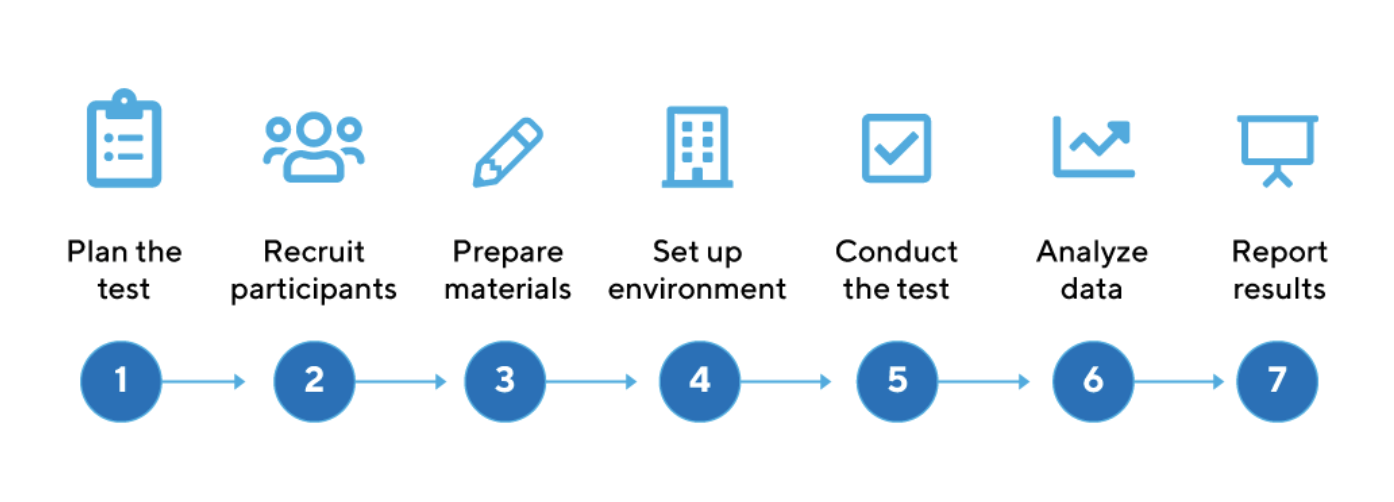
\includegraphics[width=6.5in, height=2.8in]{usability-testing.png}
\caption{Usability Test Steps}
\label{fig:usability}
\end{center}
\end{figure}
If we follow the templates and see the Embold as a test case, following are the take aways,

\begin{itemize}
\item Website is not efficient.
\item Problem in Navigation through the account and the Dash Board.
\item Hovering issues.
\end{itemize}

\section{Test tools \& Metrics}
Metrics are used to quantify the usability of any product. It is a standard which  is used to describe more than one attribute of any product. There are many secondary reasons to use the metrics i.e for a better communication with stakeholders, comparing the product with other same type of products. But the primary purpose is to yield a quality product which has considerably good user experience.
There are a number of ways we can use to test the UX design, we can use google analytics to have and educated guess and few other ways to test; number of users, their activities etc.  \par
We can utilize the concept of Behavioural and Attitudinal KPIs to measure the usability. Both these terminologies can be very briefly classified as: ~\cite{tools}
\begin{itemize}
\item Behavioural KPI (What it does)
\item Attitudinal KPI (What they say)
\end{itemize} 
Now going in detail of each of these KPIs;
\subsection{Behavioural KPI (What it does)}
It is a quite cheap way of collecting the KPIs and its kind of numerical KPI to evaluate the design. There are 4 major KPIs which fall under this category. \par
\textbf{\emph{Task Success Rate:}}\par
\indent If we talk in context of Embold, we can say its a measure of tasks completed successfully i.e, the logging in, trying to connect the Git Repository, successful scanning of the repository. 
Iff 10 people are given a task to do to test the tool, while 7 are able to do the task successfully then TSR could be calculated as :\[TSR= 7/10*100=70\%\]\par
\textbf{\emph{Time-on-task:}}\par
This KPI indicates the time spent to complete any specific task. Its actually average which is calculated considering the various tasks. Shorter the task, better the user experience. In case of the embold, I did spend much time on navigation and finding the indicators. So its user experience was not very great. \par
\textbf{\emph{Search Vs Navigation:}}\par
It is very handy if a user does not have to use SEARCH feature. So it is degree of usage of Navigation bar and Search bar. More the usage of search bar, weaker is the user experience. But in case of Embold, there is no Search Bar in the main web page, which is indication of poor user experience. Though the website has the search bar in the account inside but the UI is not of better quality as it is difficult to differentiate. \par

\textbf{\emph{User Error Rate:}}\par
The number of times any user makes the wrong entry, is considered as User Error Rate. It gives idea of how user friendly a website is.  The higher the rate of error, higher will be the usability problems. For example if a user tries to insert the date of birth in his name section, it should be an error and should be predefined, as name section should not include integers and so on. \par

\subsection{ Attitudinal KPI (What they say)}
It is about the feelings of the user, how the user feels and express their experience about the website. \par
\textbf{\emph{System Usability:}}\par
This section is kind of survey, which has 10 possible questions and 5 options to answer. It ranges from agree strongly to strongly disagree. It is not very difficult to conduct such surveys,,, because the questions are very much straight forward. I have used to the survey questionnaire to determine this KPI as shown in Figure ~\ref{fig:SUS}.\par
\begin{figure}[htbp]
\begin{center}
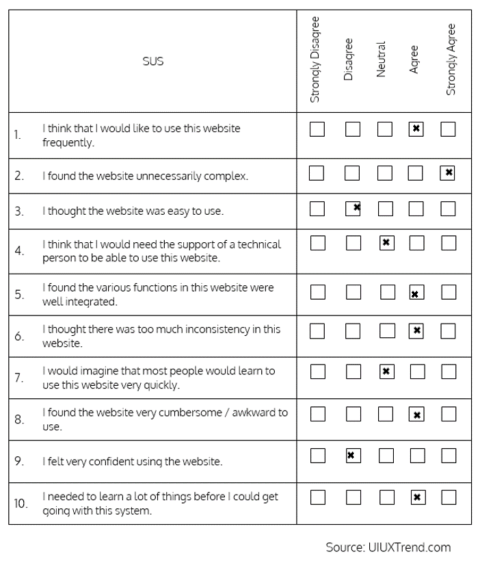
\includegraphics[width=4in, height=6in]{image.png}
\caption{System Usability Scale}
\label{fig:SUS}
\end{center}
\end{figure}
\textbf{\emph{Net Promoter Score:}}\par
It is about the referral of website, as it is just one liner question e.g ``How likely is it that you will recommend our website to the friends, colleagues etc". The answer ranges from 0-10 and categorized as:
\begin{itemize}
\item Detractors: 0 to 6
\item Passives 7 to 8
\item Promotors 9 to 10
\end{itemize}
from these 3 categories the `Passives' are ignored, and rest of the calculation goes like \[ (Number\ of\ Promoters - Number\ of\ Detractors) / (Number\ of \ Respondents) *100\]
\textbf{\emph{Customer Satisfaction:}}\par
This KPI asks about the satisfaction of the user during their experience using the website. It has normally score from 0 to 100 and divided in 5 stages i.e very dissatisfied, dissatisfied, neutral, satisfied, very satisfied. In this only the satisfied answers are considered and later percentage is taken out.  
\section{Usability Test Report}
What ever the design is, it is based on the result mentioned in Usability Test Reports. It is very important to incorporate the results mentioned in this report. There are few steps which are followed to write a comprehensive test report. Designers use this report step by step to enhance UI and UX design. The report is comprehensive and it contains the description about the problems in the design. There can be the workshops and highlight video in the comprehensive depending upon the nature of the product and its complexity. \par
Video can include the user in action and the hurdles they face in performing the tasks. While the workshop results can be part of the report. Also results are prioritized according to their level of intensity, also the graphical solutions could be the part of the report in order to help the designers how the users can be engaged. 